% !TeX encoding=utf8
% !TeX spellcheck = en-US

\section{Learnings}
\label{sec:lear}

In this section, we discuss learnings from the initial deployment of the OC platform during the first open call. We shortly present two implemented experiments, and the experimentation teams' experiences from utilizing the OC platform. In continuation, we discuss the most common issues and comments experimenters have provided regarding their experiments. Finally, we discuss architectural considerations on how to robustly scale the OC platform in future deployments.

\subsection{Experimenter Experiences}

As mentioned in the introduction, 25 experiments were conducted in five different European cities during the first open call. All experiments used the OC platform, and each experiment team was required to report on their learnings with the OC platform. These reports were conducted twice: first through an interim standardized questionnaire, and then again at the end of the experiment. In this paper, we put emphasis on those inputs provided in the final questionnaires, since they bring richer descriptions of experiences with the technical part of the OC platform, than the interim questionnaires. In the following subsections, we present two specific experiments in order to show practical examples of how the OC platform has been utilized. We then discuss the most prevalent learnings reported by all experimenters.

\subsubsection{Spend Network}

 This experiment\footnote{https://organicity.eu/experiment/spend-network-2} aimed to develop a user-friendly, online based insight analysis tool for government, citizens and SMEs in London. The objective was to improve procurement efficiency and competition. The experimenters wanted to combine their own existing data with the OC platform in order to cross-reference with new data, and to perform enhanced spending and tendering categorizations. In order to make government spendings and tendering processes visible and easily understandable, the experiment used the TinkerSpace tool\footnote{https://docs.organicity.eu/tools/tinkerspace}, the Asset Federation API\footnote{https://docs.organicity.eu/api/Federation.html} and the OC's Urban Data Observatory (UDO)~\cite{gutierrez1}. TinkerSpace is one of the tools provided by the OC platform to simplify experiment development. This tool was used for the development of an interactive smartphone application where users are provided with an intuitive overview of the categorized data. The Asset Federation API was used for adding data to the OC platform in order to enable third party developers to use such data. Furthermore, adding data to the platform made it easier to connect them to TinkerSpace, thereby reducing development complexity. Finally, UDO was used for validating that assets were actually pushed to the OC platform, and for presenting them to third-party developers.

In general, the experimenters were satisfied with the OC platform, and managed to use the services, although not always as expected. They even developed new functionalities for the TinkerSpace tool, which they made publicly available for anyone to use. Despite of the good impression, they experienced several inconveniences with the OC platform. They reported that documentation was lacking or needed to be significantly improved for external developers to properly grasp and utilize the OC platform. Understanding the services, the documentation and getting support from the OC technical team required considerable waiting periods which they deemed inefficient resource usage. In addition to documentation, they reported that access to historical data was paramount for their experiment, and it was inconvenient that the OC platform did not provide such a feature at that time. They managed to solve the issue by providing a custom persistence feature. On top of these issues, the experiment team suggested that authentication on the OC platform should be more consistent, since they had to confirm their log in every time they navigated between different portals of OC.

Final comments from this experiment team revolved around maturity level of the platform in general. They reported that the UDO needed to further develop customization, TinkerSpace needed to significantly improve the usability, and the OC platform APIs were being re-factored during the experimentation period.

\subsubsection{WearAQ}

This experiment\footnote{https://organicity.eu/experiment/wear-aq-2} utilized IoT, machine learning (ML), wearable technologies, and citizen participation for investigating human perception of air quality in cities. This was done through developing gesture recognition gloves, worn by pupils during a walk around the city. The children were taught simple hand gestures that would signify whether they felt the air was polluted or not. In parallel, the experiment team did simultaneous air quality measurements with high-quality pollution monitoring equipment. The collected data was combined with data from the OC platform, and London air quality data assets. By applying ML techniques on the generated dataset, the experimenters identified that there was a correlation between the children's perception of air quality, and the measurements of the pollution monitoring equipment. 

In order to conduct the experiment, WearAQ utilized the Asset Federation API, Asset Discovery API, Scenario Tool and the UDO. The Scenario Tool was initially used, to get inspiration on how to shape their experiment. The UDO was used for searching environmental and traffic data within confined geographical areas. The Asset Discovery API was used for extracting real-time data for their ML models. Finally, they wanted to use the Asset Federation API for inserting their refined datasets into the OC platform, so that future experimenters can work with their findings.

Even though the experiment was successful, the team reported several issues with the OC platform. In their own words, ``there was a lot of documentation'', but they reported that parts of it were missing. There were inconsistencies between different documentation pages, some cross-referencing links were broken, and it could be hard to decipher the documentation from a non-technical perspective. They mentioned that it was difficult to grasp how to format parameters when using the RESTful APIs. They suggested that it might have been easier to comprehend if more usage examples were provided in the documentation. They also reported that error messages, returned from the APIs, were unclear. Apart from documentation issues, they reported that access to historical data was a lacking feature they had expected to be part of the OC platform, and they assumed that it was possible to manually upload assets directly through the Experimenter Portal. These missing features made the experiment more cumbersome, but they did mention that support from the OC technical team was good and swift, allowing the experiment to progress. \highlighttext{As a general comment, they stated that the OC platform felt a little shaky due to multiple platform updates during the experimentation period (in order to provide new features and bug fixing).}

\subsubsection{Overall Experimenter Learnings}

As mentioned previously, 25 experiments were conducted during OC's first open call. Through a grounded theory coding approach~\cite{charmaz2006constructing}, we conducted two iterations of analyzing the evaluation questionnaires. First, we performed an initial coding by annotating relevant passages with summative descriptions. In the second iteration, we conducted focused coding thereby abstracting the descriptions into nine overarching categories~\cite{charmaz2006constructing}. We have provided the categories in \Cref{tab:arch} (in alphabetic order), and further discuss these in the remainder of this section. A detailed usability assessment is available online in \cite{d55}.

From \Cref{tab:arch}, we see that the first deployment of the OC platform did not run smoothly, and this had consequences regarding how experimenters were able to use it in their experiments. Even though several issues and inconveniences occurred during the first experimentation period, the goal never was to have a fully fledged OC platform up and running from day one. Instead, we applied an experimentally-driven approach, where we wanted to collaboratively develop the OC platform with the experimenters. 

\begin{savenotes}
\begin{table*} 
	\centering
	\caption{Experimenter Experiences}
	\begin{tabular}{p{.1\textwidth}|p{.53\textwidth}|p{.3\textwidth}}\hline\hline
		\textbf{Category} & \textbf{Summarized experiences} & \textbf{Improvements}\\\hline
		
        Bugs & Reported bugs ranged from being inconsistencies in documentation (i.e., dead links) to not being able to create data assets through the Experimenter Portal, and experiencing that private assets where publicly available for third parties. Bugs could be small and insignificant to resulting in complete lock-down of developing an experiment. This means that bugs were present in all parts of the OC platform, and most experimenters experienced those at some point. & \highlighttext{Cleaning up documentation, fixing bugs, altering existing functionality and defining new services. User and Experiment management were services heavily refactored in order to fix bugs and provide a higher degree of management granularity (see \Cref{sec:adv}).}\\\hline
		
        {Data \hyphenation{Availability} Availability} & Data within the OC platform were outdated or not available when experimenters wanted to use them. The volume of data was too small, and it was challenging to find relevant data. & \highlighttext{Improved data search through an Annotations service and a Reputation service (see \Cref{sec:adv}).}\\\hline
        
		Documentation & This category has been heavily commented throughout all evaluations, and seems to be the pivot point for most of the frustrations during the experiments. We have divided this category into seven sub-categories (ordered alphabetically):
		
        %Shink the space on top and left of the itemize 
		%\begin{itemize}[topsep=-0.5cm,leftmargin=0.3cm]
        \begin{itemize}
			\item\emph{Ambiguity}: Ambiguous API naming conventions, abbreviations and contradictory documentation has been a hindrance.
			\item\emph{Error messages}: Vague, confusing, unhelpful and generic error messages were difficult to comprehend, and no documentation, on how to interpret the messages, was provided.
			\item\emph{Examples}: More and better usage and coding examples, as well as step-by-step tutorials are desired.
			\item\emph{Improvements}: Updating documentation more often, providing high-light examples, and use the Github\footnote{https://github.com} platform features even more would be of great value.
			\item\emph{Inconsistencies}: Parts of documentation was deprecated, had dead links, and errors like references to \emph{localhost} was not corrected. Documentation could suddenly change and there was inconsistencies between different documentation.
			\item \emph{Readability}: Documentation was not easy to comprehend for a non-technical person.
			\item \emph{Unclear descriptions}: Documentation was not sufficiently elaborated and hard to follow, it was not clear how to format API parameters and it could be hard to understand how the OC services should be used and interact.
		\end{itemize}%
        %\vspace*{2mm}%Hack to shrink the space below the itemize
		 & \highlighttext{Recognizing that documentation was the main source of frustration, this part has been totally refurbished. The new documentation\footnote{https://docs.organicity.eu/} first provides a general OC platform description for experimenters to become familiar with the modules and terminology. From such description, links are provided to different parts where technical information is provided. In addition, step-by-step tutorials have been elaborated covering the most relevant and recurring procedures. Finally, the APIs documentation has been reviewed to avoid inconsistencies.}\\\hline
         
		{{Lack of~} \hyphenation{functionality}functionality} & Two features were lacking, which experimenters had expected to be available. This is API access to historical data, and the ability to provide filtering options when searching for data. & \highlighttext{Historical REST-based data API introduced during first experimentation phase, and data filtering added to the UDO. WebSocket-based service developed for providing push notifications on asset updates (see \Cref{sec:adv}).}\\\hline
        
		Positive feedback & The OC platform was well designed and the available tools were both relevant and usable. Especially the graphical data searching (the UDO) was great for getting an overview of what data was accessible through the OC platform. One experiment team reported, that the authentication and authorization functionality enabled them to have a clear division between their own custom developed software and the OC services. & \highlighttext{Annotations and Reputation services added to the UDO. Improved ability to interface directly with the OC platform APIs. Particularly evident in the User management and Annotations services.}\\\hline
        
		Suggested new functionalities & Data visualization is quite simple in the OC platform, and is reduced to showing assets on a map in a browser. Experimenters would have liked more comprehensive data visualization features in order for them to play around with the data, and it could have simplified their custom developments. It was also reported that visualizations of historical data would have been beneficial. Finally, one experiment team reported that they wanted to have more fine grained authorization configurations in the APIs in order to control who could upload data to the OC platform. & \highlighttext{The UDO was continuously expanded, and a historical data graph was added at the very end of the first experimentation phase. Fine-grained user and experiment configuration have been added through the User and Experiment management services.}\\\hline
        
		Support & Level of support was satisfactory, and direct communication via phone, email or Slack\footnote{http://slack.com} was fast and helpful. A few experimenters reported that Slack could be confusing due to multiple channels, and occasionally response times were slow. & \highlighttext{Slack has been replaced by an open forum\footnote{https://docs.organicity.eu/}, based on the Q2A\footnote{http://www.question2answer.org/} platform, in order to reduce confusion and optimize support efforts.}\\\hline
        
		Technical breakdowns & The Experimenter Portal produced error messages, changes could not be saved and invitations to participants would not be sent. The OC platform crashed regularly initially, functionality was often refactored, and experimenters had to adapt their existing codebase. When adding new assets to the platform, errors would arise when API attributes contained special characters. & \highlighttext{Errors and issues were captured and major revisions carried out including: better functionality consistency, lower coupling between platform components, updating server infrastructure and architectural considerations.}\\\hline
        
		Usability & From a usability perspective, experimenters were divided. Half of the experimenters found the OC platform easy to understand and use, while the other half found it cumbersome and unnecessary complex. The latter consisted primarily of experiment teams with a non-technical background. Regarding the UDO, most experimenters found it easy to use and helpful for understanding the concept of the OC platform. On the other hand, most experimenters had difficulties understanding and using the authentication and authorization functionality. Parts of the issues came down to understanding OAuth2. & \highlighttext{A large part of the platform revisions have been pivoting around improving usability through step-by-step examples, expanding the graphical representation of User and Experiment management, reducing the steps needed to authorize against Keycloak, only expose relevant API functionalities etc.}\\
		\hline\hline
		
	\end{tabular}	
	\label{tab:arch}	
\end{table*}	
\end{savenotes}

As a result, the first deployment of the OC platform should be perceived as a prototype of how an EaaS framework could be composed. This also means that the OC platform, as a whole, was not user-tested until it was made available to experimenters. The experimenters were aware of that the OC platform was not fully functional, and they were consequently prepared for experiencing issues. Knowing that  experimenters would encounter problems, we set up several communication pipelines (e.g., email, Slack or phone) so that experimenters could easily get in contact, and thereby progress their own developments. When issues and bugs were reported, we did our best to fix them immediately, but we had to prioritize which were most critical. As a result, some bugs were not corrected during the first experimentation period, and we suggested workarounds instead. We made sure to plan the implementation of the reported features so they would be implemented after the first experimentation period (i.e., historical data storage). According to \Cref{tab:arch}, it seems that the provided support pipelines have been satisfactory. From an internal OC perspective, support took up significantly more time than initially expected.

After the first open call ended, we significantly improved the OC platform by adding new functionalities. We have provided API access to historical data, and documentation has been significantly re-factored with updated examples, step-by-step guides and tutorials. Dead links, due to the continuous updates in the platform's documentation, have been fixed and coherency between different documentation locations has been improved.

In relation to documentation, experimenters reported this to be the culprit of most of their technical frustrations. Despite this, an interesting finding is that several experimenters reported that reading documentation and debugging took too much time, which they felt was both wasted and insufficient. We do not have specific figures on how much time experimenters actually spent on these activities, but empirical studies and our own experiences show that professional developers usually spend around 70\,$\%$ of their development time doing nothing but reading documentation and debugging~\cite{Minelli2015}. The expressed frustration was therefore a result of the non-technical nature of the experimenters participating in the open call. Since we do not have metrics for comparing time spent on actual programming, it is not possible to measure the efficiency of the OC platform's documentation, but according to the experimenters, this part took up a significant amount of their development time. In hindsight, this indicates that high quality documentation is of utter importance when exposing an EaaS platform to third-party developers.

\subsection{Architectural Considerations for Platform Scaling}

As we have commented in Section~\ref{sec:intro}, OC followed a centralized data architecture for both, storing and search. However, this approach may have scalability constraints, and hinder its adoption. In this sense, the ETSI\footnote{http://www.etsi.org} has created the Context Information Management (CIM) group, which is actively working on evolving the current definition of OMA-NGSI~\cite{NGSIOMA} and Orion Context Broker~\cite{FiwareOrion}  implementation (referred to as Orion in the remainder of this paper), developed by the FIWARE EU Initiative\footnote{https://www.fiware.org}. The preliminary technical specification of the so called NGSI-LD has recently been published~\cite{NGSILD}, and it proposes different options to deploy centralized and distributed architectures. In the following, we describe the different options that can be adopted and how they fit with the existing OC platform. 

Since we have followed a centralized approach, the different OC services access the central Orion for any data related action. As mentioned, this yields scalability limitations, and enforces to having a centralized architecture. In order to overcome such limitations, we are studying how to use NGSI-LD functionalities to enable hierarchical and distributed context information storage. \Cref{fig:arch2} provides an overview of federation with distributed storage.

Similar to the current OC architecture presented in \Cref{fig:arch}, the future approach will consider that different sites (i.e., cities) produce data that can be federated with a central OC instance. Cities will host local instances of Orion, that will be fed by context producers. Typically, the producers are services run by city service providers, that generate information which the city stores. Then, the site brokers notify the context registry about the locally stored data. Different to the current OC implementation, the registry does not store the data, but only where the data can be found. Finally, a distribution broker acts as proxy to access the data, by checking the data location in the registry. As can be observed, in this approach no data duplicates are generated, thus solving scalability issues. In addition, it is possible to replicate the same architecture at different scales, as depicted in Figure~\ref{fig:arch2}. This way, a site broker can internally act as a distribution broker. Furthermore, this approach will also enable cities to deploy local instances of OC with the required micro-services, while still being part of a larger deployment.

\begin{figure}
	\centering
	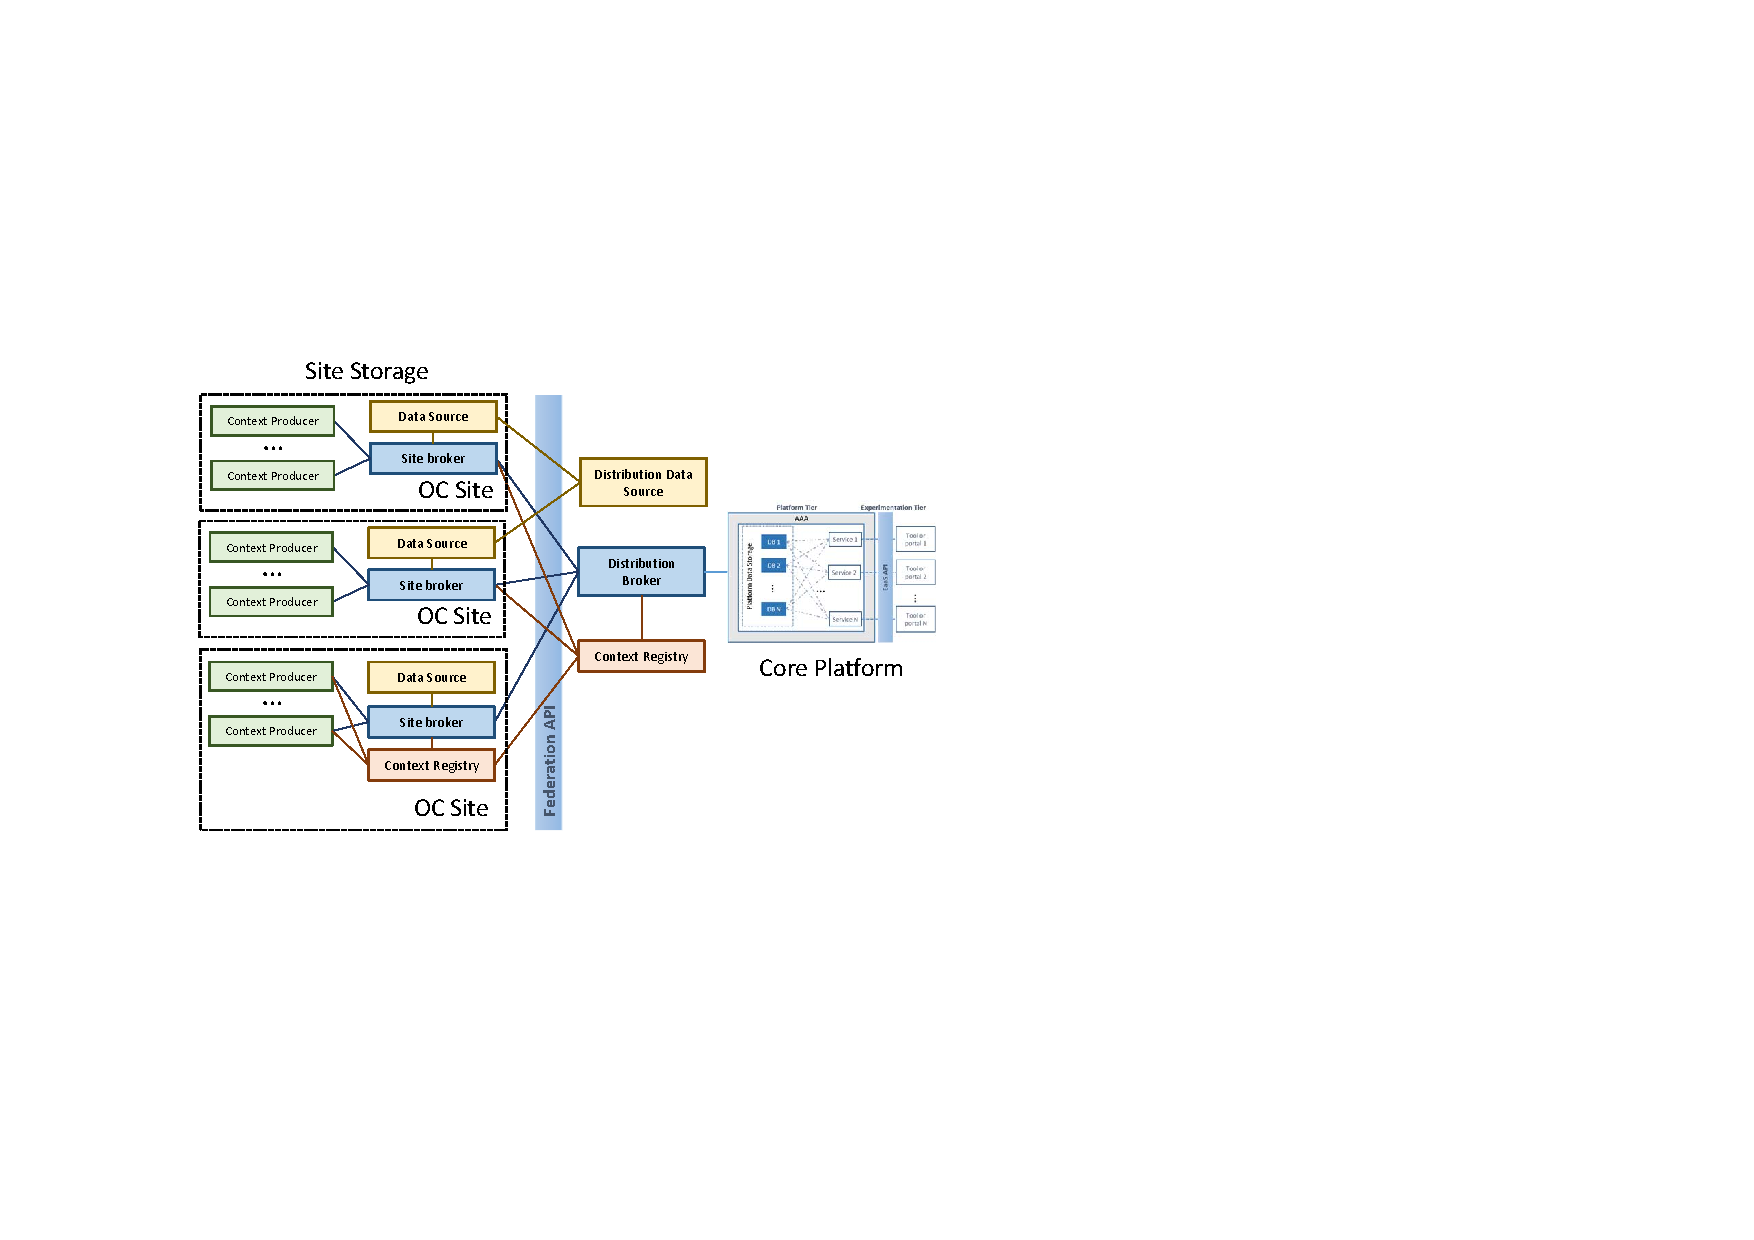
\includegraphics[width=\columnwidth]{figures/archExt}
	\caption{Distributed federation architecture}
	\label{fig:arch2}	
\end{figure}